\documentclass[12pt]{article}

\usepackage{booktabs}
\usepackage[usenames,dvipsnames]{xcolor}
\usepackage[textsize=footnotesize]{todonotes}
\usepackage[utf8]{inputenc}
\usepackage{url}
\usepackage{graphicx}
\usepackage{amssymb}
\usepackage{amsmath}
\usepackage{amsthm}
\usepackage{setspace}
\onehalfspacing
\usepackage{natbib}
\bibliographystyle{plain}
\usepackage{framed}
\usepackage[titles]{tocloft}
\setlength{\cftbeforesecskip}{0.1ex}
\renewcommand{\cftsecfont}{\rm}
\renewcommand{\cftsubsecfont}{\rm}
\renewcommand{\cftdot}{\ensuremath{\dots}}
\renewcommand{\cftsecdotsep}{3}
\renewcommand{\cftsubsecdotsep}{3}
\renewcommand{\cftsecpagefont}{\sl}
\renewcommand{\cftsubsecpagefont}{\sl}
\usepackage{sectsty}
\sectionfont{\large\it\centering}
\subsectionfont{\normalsize\it\centering}
\usepackage{listings}
\usepackage{fancyvrb}
\usepackage[margin=2cm]{geometry}
\usepackage[titletoc]{appendix}
%\usepackage{bcprules}
\usepackage{tikz}
\usepackage{pgf}
\usetikzlibrary{arrows,automata}
\usepackage{tikz-cd}
\usetikzlibrary{positioning}
% boxes around figs
\usepackage{float}
\floatstyle{boxed} 
\restylefloat{figure}


\DefineVerbatimEnvironment{code}{Verbatim}{fontsize=\footnotesize}

% Copilot + formatting for listings
\lstdefinelanguage{Copilot} {
  language = Haskell,
  morekeywords = {arg, Bool, Double, Float, Int8, Int16, Int32, Int64,
                  Word8, Word16, Word32, Word64, Spec, Stream, String,
                  Proof, Universal, Existential,
                  true, false, label, Nothing, Just, arg, constant, drop,
                  trigger, observer, prop, theorem, interpret, reify, local,
                  extern, externB, externI8, externI16, externI32, externI64,
                  externW8, externW16, externW32, externW64, externF, externD,
                  externFun, externArray, externArrayB, externArrayI8,
                  externArrayI16, externArrayI32, externArrayI64, externArrayW8,
                  externArrayW16, externArrayW32, externArrayW64, externArrayF,
                  externArrayD, not, abs, signum, complement, recip, exp, sqrt,
                  log, sin, cos, tan, asin, acos, atan, sinh, cosh, tanh, asin,
                  acosh, atanh, cast, unsafeCast, mod, div, logBase, xor, mux},
  % formatting
  commentstyle = \color{ForestGreen}\it,
  keywordstyle = \color{blue}\bf,
  literate = {+}{{$+$}}1 {/}{{$/$}}1 {*}{{$*$}}1 {=}{{$=$}}1
             {>}{{$>$}}1 {<}{{$<$}}1 {\\}{{${\color{blue}\lambda}$}}1
             {\\\\}{{\char`\\\char`\\}}1
             {\ .}{{$\circ$}}2 {\ .\ }{{$\circ$}}2
             {>>}{{>>}}2 {>>=}{{>>=}}2
             {++}{{${\color{blue}++}$}}2
             {|}{{$\mid$}}1
             {==>}{{${\color{blue}==>}$}}3
}

% A custom version of Haskell for listings
\lstdefinelanguage{Haskell} {
  morekeywords = {as, case, of, class, data, data, family, data, instance,
                  default, deriving, do, forall, foreign, hiding, if, then, else, import,
                  infix, infixl, infixr, let, in, mdo, module, newtype, proc, qualified,
                  rec, type, where},
  morecomment=[l]{--},
  morecomment=[s]{{\{-}{-\}}},
  morestring=[b]",
  literate= {'c}{{$\gamma$}}1
  {'d}{{$\delta$}}1 {'e}{{$\eta$}}1
}

%\lstnewenvironment{code}
%    {\lstset{}%
%      \csname lst@SetFirstLabel\endcsname}
%   {\csname lst@SaveFirstLabel\endcsname}
%\lstnewenvironment{Haskell}
%{
%\lstset{
%    language=Haskell,
%    basicstyle=\small\ttfamily,
%    flexiblecolumns=false,
%    basewidth={0.5em,0.45em}
%}
%}
%{}


\definecolor{mygreen}{rgb}{0,0.6,0}
\definecolor{mygray}{rgb}{0.5,0.5,0.5}
\definecolor{mymauve}{rgb}{0.58,0,0.82}

% Global listings settings
\lstset{
  basewidth={0.5em,0.45em},         % spacing more like verbatim
  basicstyle=\footnotesize\ttfamily,% the size/face of the fonts that are used for the code
  backgroundcolor=\color{white},    % choose the background color; you must add \usepackage{color} or \usepackage{xcolor}
  breakatwhitespace=false,          % sets if automatic breaks should only happen at whitespace
  breaklines=true,                  % sets automatic line breaking
  captionpos=b,                     % sets the caption-position to bottom
  commentstyle=\color{mygreen},     % comment style
  %deletekeywords={ls,xor,conj,reset,gt,input},            % if you want to delete keywords from the given language
  escapeinside={\%*}{*)},           % if you want to add LaTeX within your code
  extendedchars=true,               % lets you use non-ASCII characters; for 8-bits encodings only, does not work with UTF-8
  frame=single,                     % adds a frame around the code
  keepspaces=true,                  % keeps spaces in text, useful for keeping indentation of code (possibly needs columns=flexible)
  keywordstyle=\color{blue},        % keyword style
  rulecolor=\color{black},          % if not set, the frame-color may be changed on line-breaks within not-black text (e.g. comments (green here))
  showspaces=false,                 % show spaces everywhere adding particular underscores; it overrides 'showstringspaces'
  showstringspaces=false,           % underline spaces within strings only
  showtabs=false,                   % show tabs within strings adding particular underscores
  stringstyle=\color{red},          % string literal style
  tabsize=2,                        % sets default tabsize to 2 spaces
}


\newtheoremstyle{example}{\topsep}{\topsep}
     {\normalsize\sl} % Body font.
     {}               % Indent amount (empty = no indent, \parindent = para indent).
     {\small\it}      % Thm head font.
     {:}              % Punctuation after thm head.
     {\newline}       % Space after thm head (\newline = linebreak).
     {\thmname{#1} \thmnumber{#2}\thmnote{#3}} % Thm head spec.
\theoremstyle{example}
\newtheorem{example}{Example}

\newcommand{\hlinepage}{\rule{\textwidth}{0.25pt}}
\newcommand{\HRule}{\rule{\linewidth}{0.25pt}}
\newcommand{\fixme}[1]{\emph{\color{Red}\{!~#1~!\}}}

\begin{document}

\thispagestyle{empty}

\begin{center}

University of Missouri / ENS Paris / Galois Inc. / NASA LaRC

\vspace{0.1cm}

\HRule

\vspace{0.6cm}

{\Huge \bfseries
Assured Runtime Verification }
\HRule

\vspace{0.6cm}
\begin{minipage}{0.3\textwidth}
\large
\begin{center}
Chris Hathhorn \\
\small{
hathhorn@gmail.com\\
}
\end{center}
\end{minipage}
\begin{minipage}{0.3\textwidth}
\large
\begin{center}
Georges-Axel Jaloyan \\
\small{
georges-axel.jaloyan@ens.fr\\
}
\end{center}
\end{minipage}

\vspace{1cm}

\begin{minipage}{0.3\textwidth}
\large
\begin{center}
Lee Pike\\
\small{
leepike@galois.com\\
}
\end{center}
\end{minipage}
\vspace{1cm}


\begin{minipage}{0.3\textwidth}
\large
\begin{center}
Alwyn E. Goodloe\\
\small{
a.goodloe@nasa.gov\\
}
\end{center}
\end{minipage}
\vspace{1cm}

{\large
Hampton, Virginia, United States, \today
}

%\begin{tabular}{cc}
%\hspace{0.5cm}\includegraphics[width=0.18\textwidth]{figures/nia}\hspace{0.5cm}  &
%\hspace{0.5cm}\includegraphics[width=0.2\textwidth]{figures/galois}\hspace{0.5cm} &
%\hspace{0.5cm}\includegraphics[width=0.2\textwidth]{figures/nasa}\hspace{0.5cm} \\
%\textsc{\large NIA} &
%\textsc{\large Galois Inc.} &
%\textsc{\large NASA LaRC} \\
%\end{tabular}


\end{center}

\vspace{0.25cm}

\section*{Abstract}
{
\small We descirbe an approach to assured runtime verificaition. Our apporach is illustrated using an example from airspace management.
}

{
\small
\setcounter{tocdepth}{2}
\tableofcontents
}

\newpage
\addcontentsline{toc}{section}{Acknowledgement}
\section*{Acknowledgement}
TBD
{
\section{Introduction}~\label{sec:intro} 

The consequences of failure of safety-critical systems such as nuclear
reactor shutdown systems, railway switching systems, and civil air
transportation are considered especially dire. The prescribe safety
margin of a catastrophic fault for avionics in civil aircraft is
$10^{-9}$ or one in a billion.  The justification for the requirement
is to show that failures resulting in a catastrophic effect are ``so
unlikely that it is not anticipated to occur during the operational
life of an entire system or fleet''\cite{FAA2000}.  The safety record
in civil aviation has been so outstanding the last several decades
that it is often considered the gold standard for engineering safe and
reliable systems. Strict certification regime imposed on hardware and
software as well as licensing requirements on human operators in the
system is a significant factor in the .  New technologies can take
many years to transition onto civil aviation due to the need to
demonstrate that safety is not being negatively impacted. Yet
technological advances are enabling the development of increasingly
autonomous (IA) unmanned aircraft systems (UAS) that modify their
behavior in response to the external environment and learn from their
experience.  In practice, the certification of avionics software
relies heavily on it being predicable and existing standards do not
have provisions to assure systems whose behavior is not predicable
during certification.  The US National Academies study ``Autonomy
Research for Civil Aviation''~\cite{NRC14} identifies the verification
and validation of IA systems as considerable hurdle to the adaption.


% Federal Aviation Administration (FAA) regulations
%govern the certification of aircraft and engines including the
%software. 
%Strict government regulations
%govern everything from the certification of aircraft to the management
%of the airspace . 

Runtime verification (RV), where monitors detect and respond to
property violations at runtime, has the potential to enable the safe
operation of safety-critical systems that are too complex to formally
verify or fully test using conventional test such as IA systems. The
\emph{Simplex Architecture}~\cite{simplex} provides an architectural
pattern. A monitor checks that the executing system under observation
(SUO) satisfies a specification and If the property is violated, the
RV system will the switch to system to the control of a more
conservative component that can be assured using conventional means
that \emph{steers} the system into a safe state.   


Since 2007, my colleague Lee Pike and I, with considerable help for a
bevy of talent students, have been working on program aimed at
creating a framework for \emph{high assurance RV} of safety-critical
hard real-time systems primarily in the context of the Copilot RV
framework.  In order to be used in ultra-critical environments,
high-assurance RV must:
\begin{enumerate}
\item \label{req:a} Provide evidence for a safety case that the RV
  enforces safety guarantees.
\item \label{req:d}  Be reliable in the presence of faults.  
\item \label{req:b} Support verification that the specification of the monitors
  is correct.
\item \label{req:c} Ensure that monitor code generated implements the specification of the
monitor.
\end{enumerate} 
In addition to building the Copilot framework, we have
been conducting a number of case studies.


\paragraph{Contributions} 
A considerable challenge his been discovering what were the right
questions to ask for assured RV.  This  paper is organized around a
series of questions that we feel anyone trying to apply RV in
ultracrtical IA systems must address. We will discuss how these
questions have been addressed in the context of Copilot. While far
from being a complete, we  believe
that these questions can aide others in the RV community in building
their own frameworks or conducting case studies. In keeping with the
theme of the workshop, we will highlight our use of static analysis
tools in the hope that we will not only encourage others in the
community to apply them in their own RV frameworks, but encourage the
static analysis community to collaborate with the RV researchers in
creating tools that will enable assured RV.

%Although building a safety
%case~\ciite{Kelly98arguingsafety} in the spirit
%of Rushby's~\cite{rvRushby,RushbyAIAA09} remains a challenge,  we
%believe that 
 

%To achieve this, the
%system must be architected so that the RV component can observe the
%state of the system  and prevent the autonomous decision making form
%taking unsafe actions. 





 


\section{Copilot RV Framework}~\label{sec:Copilot}

% A short introduction to the copilot language and framework.

Copilot is a language tailored to developing runtime monitors for hard
real-time, distributed, reactive systems. Briefly, a runtime monitor is a
program that runs concurrently with a target program with the sole purpose of
assuring that the target program behaves in accordance with a pre-established
specification\citep{monitors}. Copilot is a language for writing such
specifications\citep{copilot, pike-icfp-12, pike-isse-13}. It is an embedded
domain-specific language, hosted in the lazy functional programming language
Haskell.


	\begin{figure}[ht!]
		\centering
		\footnotesize
		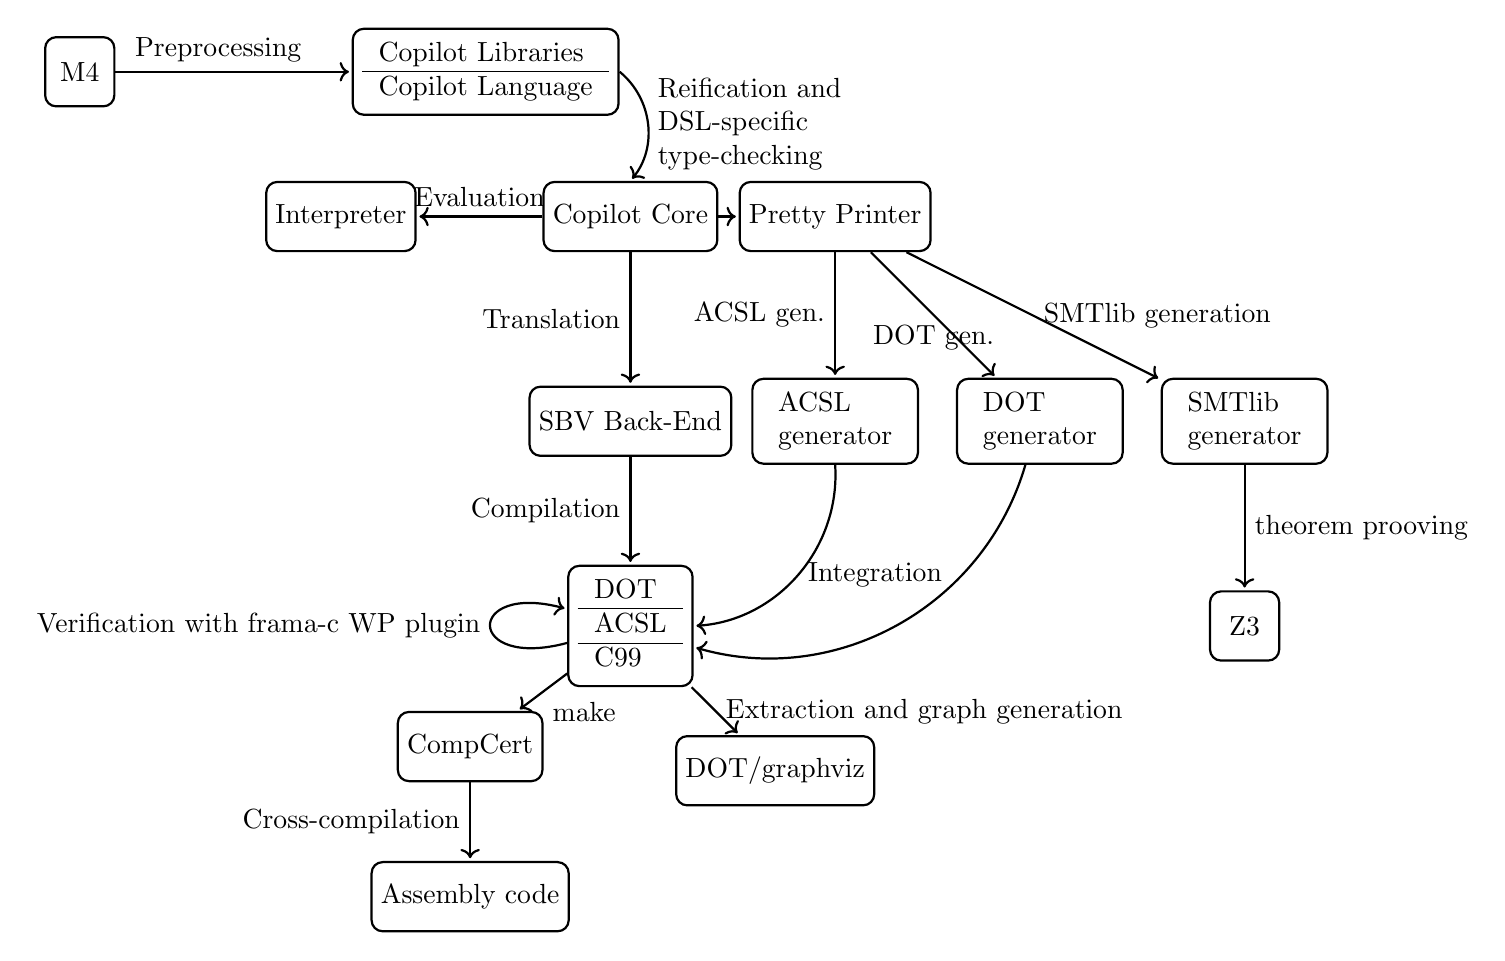
\begin{tikzpicture}[->, node distance=2.6cm, auto, shorten >=1pt, bend angle=45,
		thick]
		\tikzstyle{every state}=[rectangle, rounded corners]
		
		
		\node[state] (Int) {Interpreter};
		\node[state] (Lang) [above right of=Int]
		{
			\begin{tabular}[b]{l}
			Copilot Libraries\\ \hline Copilot Language
			\end{tabular}};
		
		\node[state] (M4) [left=3cm of Lang] {M4};
		\node[state] (Core) [below right of=Lang] {Copilot Core};
		\node[state] (PP) [right of=Core] {Pretty Printer};
		
		
		\node[state] (ACSL) [below of=PP] {\begin{tabular}[b]{l}
			ACSL\\ generator
			\end{tabular}};
		\node[state] (DOTc) [right of=ACSL] {\begin{tabular}[b]{l}
			DOT\\ generator
			\end{tabular}};
		\node[state] (SMTlib) [right of=DOTc] {\begin{tabular}[b]{l}
			SMTlib\\ generator
			\end{tabular}};
		\node[state] (Z3) [below of=SMTlib] {Z3};
		\node[state] (SBV) [below of=Core] {SBV Back-End};
		\node[state] (C99S) [below of=SBV] {\begin{tabular}[b]{l}
			DOT\\ \hline ACSL\\ \hline C99
			\end{tabular}};
		\node[state] (DOT) [below right of=C99S] {DOT/graphviz};
		\node[state] (CCOMP) [below left=0.3cm and 0.3cm of C99S] {CompCert};
		\node[state] (ASM) [below=1cm of CCOMP] {Assembly code};
		
		
		\tikzstyle{every node}=[]
		
		
		\path %% (Libs) edge node {0,1,L} (Lang);
		(Lang) edge [bend left, anchor=west, text width=2.5cm] node {Reification and DSL-specific type-checking} (Core)
		(M4) edge [text width=2.5cm] node {Preprocessing} (Lang)
		(Core) edge [anchor=east] node {Translation} (SBV)
		edge node {} (PP)
		edge node [swap] {Evaluation} (Int)
		(ACSL) edge [bend left, anchor=west] node {Integration} (C99S)
		(DOTc) edge [bend left, anchor=east] node {} (C99S)
		%(Int) edge [<->, bend right, anchor=east] node {QuickCheck} (SBV)
		(PP) edge [->, anchor=east] node {ACSL gen.} (ACSL)
		(PP) edge [->, anchor=north] node {DOT gen.} (DOTc)
		(PP) edge [->, anchor=west] node {SMTlib generation} (SMTlib)
		(SMTlib) edge [->, anchor=west] node {theorem prooving} (Z3)
		(C99S) edge [->, anchor=north west] node {make} (CCOMP)
		(CCOMP) edge [->, anchor=east] node {Cross-compilation} (ASM)
		(C99S) edge [loop left, ->, anchor=east] node {Verification with frama-c WP plugin} (C99S)
		(C99S) edge [->, anchor=west] node {Extraction and graph generation} (DOT)
		(SBV) edge [->,anchor=east] node {Compilation} (C99S);
		\end{tikzpicture}
		\caption{The new Copilot toolchain. }
		\label{fig:New toolchain}
	\end{figure}

\section{Well Clear}~/label{sec:wellclear}  

Overview of well clear. Probably summarize Cesar's papers on the subject.
Some basic formulas : \newline
$WCV_{t_{\mathrm{var}}} (\mathbf s,s_z,\mathbf v,v_z) \equiv \mathrm{Horizontal\_WCV_\mathit{t_{\mathrm{var}}}}(\mathbf{s},\mathbf v) ~\mathrm{and}~ \mathrm{Vertical\_WCV}(s_z,v_z)$ \newline
$\mathrm{Horizontal\_WCV_\mathit{t_{\mathrm{var}}}}(\mathbf{s},\mathbf v) \equiv \Vert \mathbf s \Vert \leq \mathrm{DTHR} ~ \mathrm{or} ~ 
(d_{\mathrm{cpa}}(\mathbf s, \mathbf v)  \leq \mathrm{DTHR} ~ \mathrm{and} ~ 0 \leq t_{\mathrm{var}}(\mathbf s, \mathbf v) \leq \mathrm{TTHR})$\newline
$\mathrm{Vertical\_WCV}(s_z,v_z) \equiv \vert s_z \vert \leq \mathrm{ZTHR} ~\mathrm{or}~ 0 \leq t_{\mathrm{coa}}(s_z,v_z) \leq \mathrm{TCOA}$\newline
$d_{\mathrm{cpa}} (\mathbf s, \mathbf v) = \Vert \mathbf s + t_{\mathrm{cpa}}(\mathbf s, \mathbf v) \mathbf v \Vert$ \newline
$t_{\mathrm{coa}}(s_z,v_z) \equiv \left\{
\begin{array}{ll}
- \frac{s_z}{v_z} & \mathrm{if} ~ {s_z}{v_z} < 0\\
- 1  & \mathrm{otherwise}
\end{array}
\right. $ \newline 
\newline 

With : \newline 
$\tau(\mathbf{s},\mathbf v) \equiv \left\{
\begin{array}{ll}
- \frac{\mathbf{s}^2}{\mathbf{s} \cdot \mathbf{v}} & \mathrm{if} ~ \mathbf{s} \cdot \mathbf{v} < 0\\
- 1  & \mathrm{otherwise}
\end{array}
\right. $\newline 
$t_{\mathrm{cpa}}(\mathbf{s},\mathbf v) \equiv \left\{
\begin{array}{ll}
- \frac{\mathbf{s} \cdot \mathbf{v}}{\mathbf{v}^2} & \mathrm{if} ~ \mathbf{v} \neq 0\\
0  & \mathrm{otherwise}
\end{array}
\right. $\newline 
$\tau_{\mathrm{mod}}(\mathbf{s},\mathbf v) \equiv \left\{
\begin{array}{ll}
\frac{\mathrm{DTHR}^2-\mathbf{s}^2}{\mathbf{s} \cdot \mathbf{v}} & \mathrm{if} ~ \mathbf{s} \cdot \mathbf{v} < 0\\
-1  & \mathrm{otherwise}
\end{array}
\right. $ \newline
$t_{\mathrm{ep}}(\mathbf{s},\mathbf v) \equiv \left\{
\begin{array}{ll}
\Theta (\mathbf{s},\mathbf{v}, \mathrm{DTHR}, -1) & \mathrm{if} ~ \mathbf{s} \cdot \mathbf{v} < 0 ~\mathrm{and}~ \Delta(\mathbf{s},\mathbf v, \mathrm{DTHR}) \ge 0\\
-1  & \mathrm{otherwise}
\end{array}
\right. $ \newline
$\Theta (\mathbf{s},\mathbf{v}, D, \epsilon) \equiv \frac{-\mathbf{s}\cdot\mathbf{v} + \epsilon \sqrt{\Delta(\mathbf{s},\mathbf{v},D)}}{\mathbf{v}^2}$\newline
$\Delta(\mathbf{s},\mathbf{v},D) \equiv D^2\mathbf{v}^2 - (\mathbf{s}\cdot\mathbf{v}^{\perp})^2 \\
\Leftrightarrow \Delta(\mathbf{s},\mathbf{v},D) \equiv D^2\mathbf{v}^2 - Det(\mathbf{s},\mathbf{v})^2$ 
\section{Assuring Specifications}~\label{sec:specverify}

How we assure our specfications using SMT based tools. 


\subsection{Assured Well Clear}~\label{sec:verifiywc} 

How we applied Z3 to assure WC spec.



\section{Verified Monitors}~\label{sec:vermon} 

How we leverage the Frama-C deductive verification plug-in wp to verify that the C monitors do indeed implement the high-level monitors.

Discuss tracability and  the use of Frama-C value analysis tool as well. 

\subsection{Well Clear Monitor Example}~\label{sec:verwcmon} 

Examples from the well clear monitors. 
 
\section{Turtles All The Way Down}~\label{sec:compcert}

How we leverage the compcert compiler when possible. 



\section{Flight Test}~\label{sec:flighttest} 

Here we describe our flight tests.


\section{Future Work and Conclusion}\label{sec:conclusion}

 Ultra-Critical systems are quickly evolving in complexity, and assured
 RV is a necessary complement to traditional assurance techniques.  
In this paper, we have presented the development of
\texttt{Copilot-Kind} that enhances the Copilot RV framework with an
integrated model-checking capability for verifying monitors and
illustrated its applicability to verify a range of monitors.


The development of \texttt{copilot-kind} has reinforced the efficacy
of the embedded DSL approach. Being embedded in a higher-order
functional language facilitated the creation of a number of features
such as our proof scheme capability. We have also found it quite
advantageous to be able to write properties in the familiar style of
Haskell programs. For instance, in Section~\ref{sec:mvote}, the
function \texttt{forAllCst} for the serial Boyer-Moore example in that
it uses both a \texttt{fold} and a \texttt{map} operator to model
finite conjunctions.  Beyond our own purposes, we believe that other
embedded DSL developers could use our designs in order to interface
their languages with proof engines.

Verified  monitors are by no means sufficient for achieving assured RV,
since a safety case is far more encompassing, but it is a necessary
<<<<<<< HEAD
condition.  Having applied our tool to rather
sophisticated monitors,  future extensions are planned.  Of particular
interest is an interface to 
MetiTarski~\cite{AkbarpourPaulson}. This would allow us to discharge
proofs of invariants involving real-valued special functions, which
would arise quite often in the domain of cyber-physical systems.

\subsubsection{Assurance} The reported efforts have
primarily focused on verifying invariant properties of monitors using
$k-$induction. Our solution is not a panacea as any model checking
solution is subject to the well known state explosion problem, but 
the results in verifying both simple and relatively complex monitors
are promising. 

\subsubsection{Efficacy of the Embedded DSL Approach} First, we have
demonstrated that the embedded DSL approach is powerful and flexible
in that we were able to extend the Copilot RV framework with
verification capabilities. Being embedded in a  higher-order functional language
facilitated the creation of  a number of features such as our proof
scheme capability. The fact Copilot is a Haskell based eDSL yielded
very  concise properties. For instance, in Section~\ref{sec:mvote}
the power of higher-order expression is well illustrated in 
function  \texttt{forAllCst} for the
serial Boyer-Moore example in that it  uses both a  a \texttt{fold}
and a \texttt{map} operator to model finite conjunctions. 


\subsubsection{Future Work} In the near term, we continue our
collaboration with the Kind2 team as the prover gets more
sophisticated and provides a more flexible interface. Given we already
output SMTLib format in order to interface with Yices, we will
investigate connecting to other provers that use that input
format. Finally, we shall interface the verification with
MetiTarski~\cite{AkbarpourPaulson}, which would allow us to discharge
proofs of invariants involving real-valued special functions.


\bibliography{paper}
}

%\begin{appendices}
%\end{appendices}
\end{document}

